\section{Local Halo}~\label{study-localhalo}
LocalHalo was a startup based in London who made a social network for neighbours~\footnote{\url{https://ain.ua/en/2019/10/18/localhalo-raises-500k/}} with developers in Ukraine, London, and Kazakhstan.~\citep{karpenko2019_localhalo_a_social_network_for_neighbors}. 
Table~\ref{tab:local_halo_anaytics_overview} provides an overview of this case study

{\renewcommand{\arraystretch}{0.8}% Tighter
\begin{table}[htbp!]
    \centering
    \small
    \setlength{\tabcolsep}{1pt}
    \begin{tabular}{ll}
       % Question &Answer  \\
       \toprule
       Website &\url{https://www.localhalo.com/} \\
       Founded &2018 \\
       Business Domain &Digital neighbourhood groups in UK.\\
       Business type &Startup, two co-founders: CEO and CTO \\
       Technologies  &React Native for cross-platform Android and iOS development \\
       &Expo development framework \\
       Source code  &Closed and not available for research \\
       Analytics used by team &Sentry, Mixpanel, Google Play Console \\
       Development Practices &Not explicit, a small distributed team \\
       \midrule
       User base &7,000 registered users, 1k to 2k monthly active (Jan 2020) \\
       Installations &1,000's for the Android app \\
       \midrule
       Research methods &Interview, email discussions, bug analysis, use of mobile analytics \\
       Analytics collected &Live access to: Sentry, Google Play Console with Android Vitals \\
       Research software &Vitals-Scraper used to preserve results \\
       Additional data collected &Interview notes and emails \\
       Active period &Jan 2020 to June 2020 \\
       \bottomrule
    \end{tabular}
    \caption{Case Study key facts: LocalHalo}
    \label{tab:local_halo_anaytics_overview}
\end{table}
}

The aims and objectives of this case study include:
\begin{itemize}
    \item \textbf{A startup case study}: how a small startup with a distributed team chose to incorporate mobile analytics into their product and working practices.
    \item \textbf{Their perspectives on mobile analytics tools}: They used three mobile analytics tools, each for distinct purposes. 
    \item \textbf{Mobile Analytics for cross-platform apps}: Including the opportunity to research Sentry Mobile Analytics. 
\end{itemize}

This case study contributed to several of the six perspectives; primarily to the developer's perspective on the their use of mobile analytics, and to understanding the status quo of mobile analytics tools.


\subsection{LocalHalo: Background - How the case study came about}
The case study was started through initial discussions with the CEO, James Routledge, in November 2019. He arranged for the CTO, Andriy Marin, to have a discussion to agree on how they could help and participate in this research. This discussion was an online call on \nth{17} Jan 2020 where we agreed on the scope, etc. Two pages of \emph{ad-hoc} handwritten notes were made during the call, and a summary was written up and emailed to them of what was agreed during the call. They responded and confirmed they data and findings couple be used as part of this research.

The CTO provided access to two of the three mobile analytics services; these two were Google Play Console with Android Vitals and Sentry~\footnote{\url{https://sentry.io/welcome/}}, which was used to track technical issues with their app and website. We agreed the research would not have access to the third analytics service, mixpanel~\footnote{\url{https://mixpanel.com/}}, which they used for user behaviour and related analytics. This service included personally identifiable information of their users and would not be useful for this research. We also agreed no access would be provided to the source code as that was deemed sensitive. 

\subsection{LocalHalo: development microcosm}
The development team used the Expo development platform \url{https://expo.dev/} to create native apps that ran on Android and iOS apps. These apps were released on Google Play and Apple's App Store respectively. The CTO was actively involved in writing and maintaining the source code and was supported by developers in three locations, in the Ukraine, London, and Kazakhstan.~\citep{karpenko2019_localhalo_a_social_network_for_neighbors}. 

Little additional information was available in terms of their development or release practices for their mobile apps. One observation is Expo claims to automate the release process to the app stores so the LocalHalo development team may have relied and used the Expo service.

\subsection{LocalHalo: applying analytics to the development practice}
Localhalo incorporated two analytics libraries into their cross-platform mobile application: Sentry for crash reporting and Mixpanel for business-oriented usage analytics. For their Android app they also had access to Google Play Console.

They seldom used Google Play Console with Android Vitals, it did not suit apps developed in React Native as the crashes did not actually crash the shell app which wraps the React Native app~\footnote{Note, other developers have asked about this behaviour, for instance on StackOverflow \href{https://stackoverflow.com/questions/66166824/native-crash-reporting-for-expo-deployed-to-android/}{Native crash reporting for Expo deployed to Android?}} 
(which is what appears to be monitored by Android). The shell app restarts the React Native app automatically.

The development chose to use separate analytics services for user behaviour analytics (Mixpanel) and issues such as crashes and anomalies (Sentry). Presumably the respective SDKs were incorporated into the React Native source code~\footnote{Some of the errors reported by Sentry indicate the integration used TypeScript (which is supported in React Native, see \url{https://reactnative.dev/docs/typescript}. Mixpanel also provides an opensource wrapper that supports React Native \url{https://github.com/mixpanel/mixpanel-react-native}.}~\footnote{Note: they also incorporated Sentry into their website and provided access to Sentry for their website, however the website is out of scope for this research and will not be considered further here.}. Only two people have access to Sentry: the CTO and me, therefore any other members of the development team would have indirect access, for instance via screenshots and/or bug reports raised by the CTO. 

They saw value in using analytics to improve business results, for instance for App Store Optimisation to improve the ranking of their app in the app stores. The CTO made a key observation during the interview \emph{``If you have lots of crashes you have zero chance of being promoted [by the app store]."}

In terms of user experience analytics the CTO also observed \emph{``To improve user retention you need to do both, eliminate the bad stuff [and] improve the good stuff [to] increase value"}.

The overall impression was the team had decided to incorporate mobile analytics to help them provide a reliable and valuable service for their current and hoped-for users where the team would address errors on an \emph{ad-hoc} basis.

\subsection{LocalHalo: Experiences of using mobile analytics}
They experience numerous crashes reported by Sentry, which occur within the React Native runtime environment. In March and April 2020 high failure rates were also reported in Google Play Console and Android Vitals. Figure \ref{fig:localhalo-android-vitals-no-data-16-march-2020} was recorded on \nth{16} March 2020 before these started and shows the App Health Overview page with a link to a video introducing Android Vitals~\footnote{This appears as a mainly black rectangle in this thumbnail screenshot.}, and the App Health Details page with no data.

\begin{figure}[htbp!]
\centering
\begin{minipage}{.45\textwidth}
  \centering
  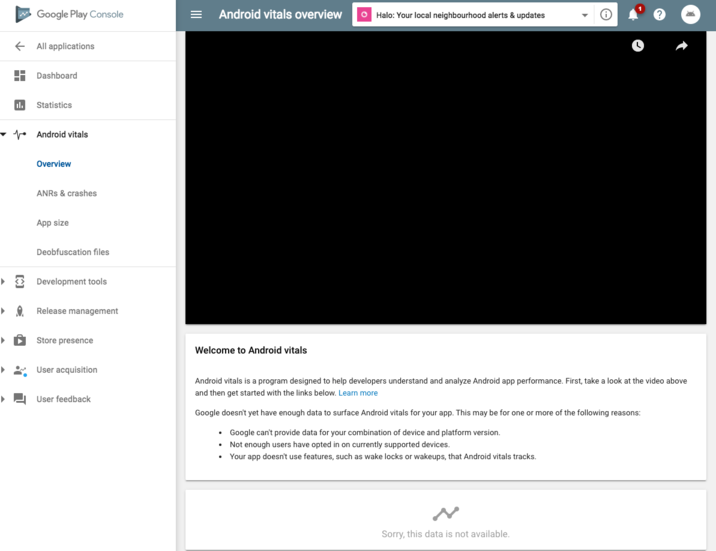
\includegraphics[width=\textwidth]{images/localhalo/apphealthoverviewplace_5550596_no_data.png}
  \captionof*{figure}{App Health Overview page}
\end{minipage}\hfill%
\begin{minipage}{.45\textwidth}
  \centering
  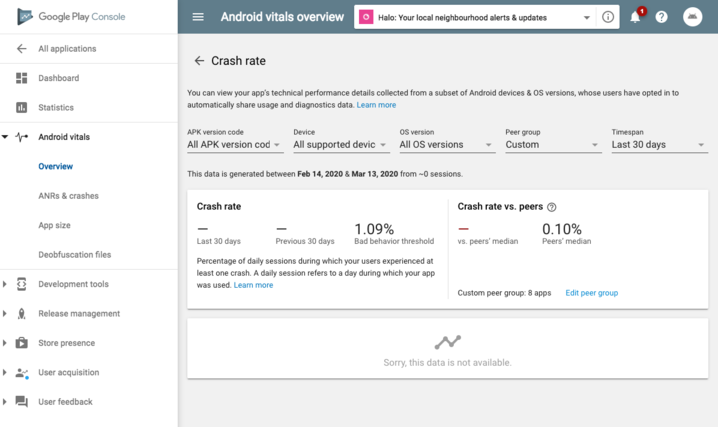
\includegraphics[width=\textwidth]{images/localhalo/apphealthdetailsplace_55505963_no_data.png}
  \captionof*{figure}{App Health Details page}
\end{minipage}
    \caption{No Android Vitals reports on \nth{16} March 2020}
    \label{fig:localhalo-android-vitals-no-data-16-march-2020}
\end{figure}

Figure~\ref{fig:localhalo-android-vitals-high-failures-26-march-2020} was recorded ten days later in \nth{26} March 2020 and shows the alerts for both high crash and ANR rates in the App Health Overview page and the graph for the rampant crash rate in the corresponding App Health Details page. These indicate the failures were related to the native runtime rather than within the React Native code. These were not reported by any Sentry Alerts and they do not appear in the weekly summary reports, except potentially by the absence of data shown in Figure~\ref{fig:sentry-missing-data-march-2020}; perhaps the error was so severe it prevented Sentry's SDK from reporting any data?

\begin{figure}[htbp!]
\centering
\begin{minipage}{.45\textwidth}
  \centering
  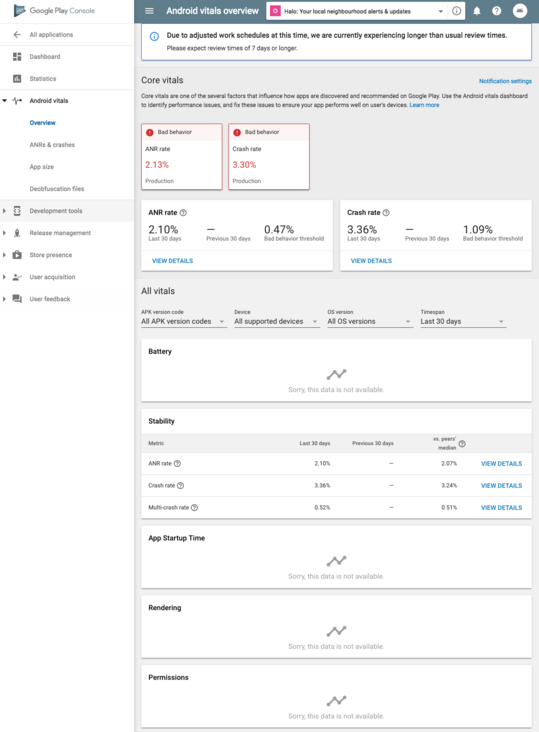
\includegraphics[width=\textwidth]{images/localhalo/apphealthoverviewplace_5550596_high_errors.png}
  \captionof*{figure}{App Health Overview page}
\end{minipage}\hfill%
\begin{minipage}{.45\textwidth}
  \centering
  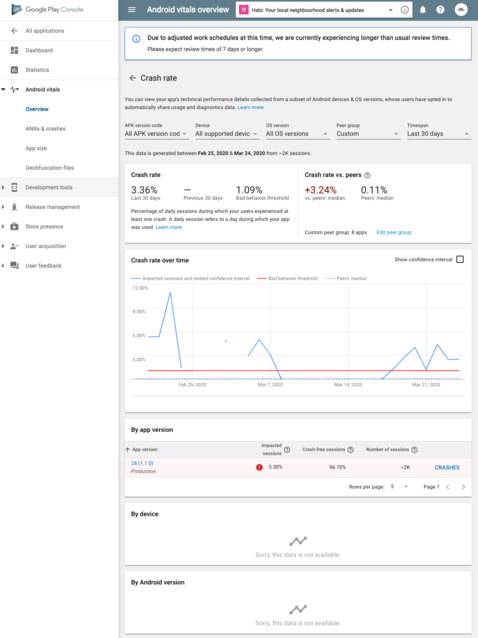
\includegraphics[width=\textwidth]{images/localhalo/apphealthdetailsplace_55505963_high_errors.png}
  \captionof*{figure}{App Health Details page}
\end{minipage}
    \caption{Alerts and graphs in Android Vitals on \nth{26} March 2020}
    \label{fig:localhalo-android-vitals-high-failures-26-march-2020}
\end{figure}
A release in March 2020 had a high crash rate for the production release of their Android app. The top crash cluster was for:

{\small \texttt{java.lang.RuntimeExceptionhost.exp.exponent.experience.a\$b.run}} 

This was traced to a problem in the expo library the development team used in the app~\url{https://github.com/expo/expo/issues/5839}~\footnote{Expo is a very popular opensource platform for making universal native apps that run on Android, iOS, and the web \url{https://github.com/expo/expo}.}. In that issue several developers for different Android apps provide data from Google Play Console confirming they also receive similar crash clusters. The cause has not yet been definitively traced or addressed, however for the LocalHalo app the crashes stopped being reported once a new release of the Android app, release 1.3.0, was released around \nth{6} April 2020.

In this GitHub issue, 5839, one of the contributors reported their app's crash rate had gone from below 1\% to 10\%~\footnote{\url{https://github.com/expo/expo/issues/5839\#issuecomment-571271045}} and that users were writing terrible reviews. Another contributor observed that the stack trace in Android Vitals is not very useful, what's needed is the error message that appears in the device's log immediately before the stack trace~\footnote{\url{https://github.com/expo/expo/issues/5839\#issuecomment-583838280}}; \phantomsection
\textbf{insight} the stack trace is not always sufficient to understand the failure\label{insight-expo-stack-trace-not-sufficient-to-identify-the-failure}.

\begin{figure}[htbp!]
\centering
\begin{minipage}{.45\textwidth}
  \centering
  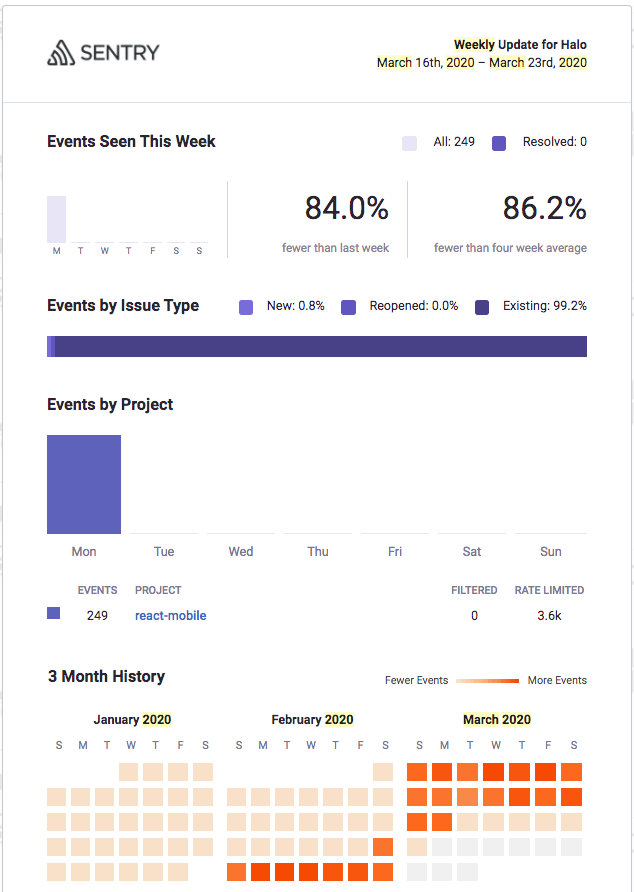
\includegraphics[width=\textwidth]{images/localhalo/sentry-weekly-report-16-mar-2020.png}
  \captionof*{figure}{\nth{16} -~\nth{22} March 2020}
  \label{fig:localhalo-sentry-weekly-report-16-mar-2020}
\end{minipage}\hfill%
\begin{minipage}{.45\textwidth}
  \centering
  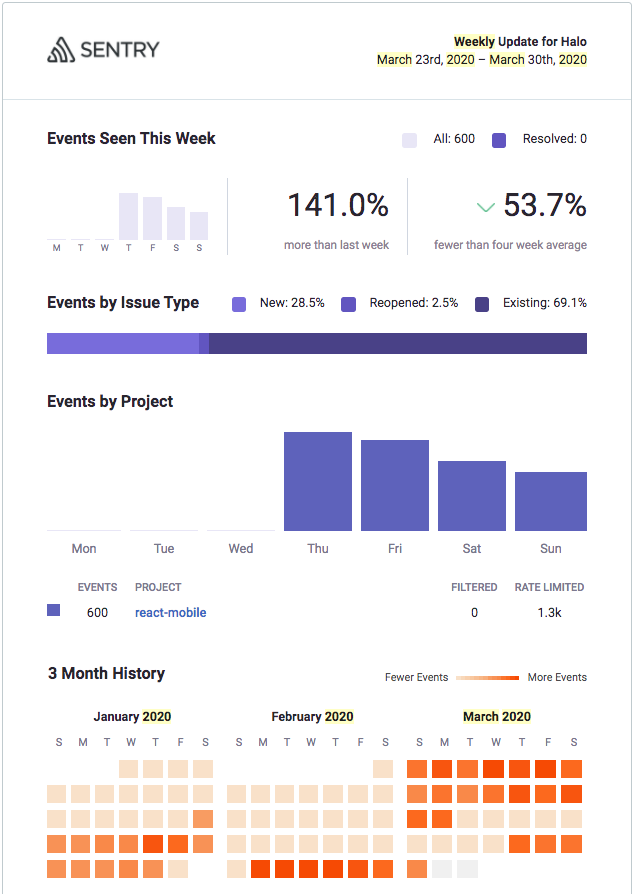
\includegraphics[width=\textwidth]{images/localhalo/sentry-weekly-report-23-mar-2020.png}
  \captionof*{figure}{\nth{23} -~\nth{29} March 2020}
  \label{fig:localhalo-sentry-weekly-report-23-mar-2020}
\end{minipage}
    \caption{Missing data reported in Sentry, in March 2020}
    \label{fig:sentry-missing-data-march-2020}
\end{figure}


\subsection{LocalHalo: data collected and methods used for collection}
This case study combines three immediate sources of data: separate meetings with the founders, email conversations, and online access to two mobile analytics tools. It also includes over 240 automated emails from Sentry's hosted mobile analytics service. Vital Scraper was also used to collect reports and crash details from Google Play Console with Android Vitals.

\newthought{Meetings with the founders}

The first meeting with the CEO was online as he was in New York, USA at the time, and the second was in person in Central London. Their main contribution in terms of the research was to enable this case study to happen. The CEO arranged a subsequent meeting with the CTO which was online and this meeting was where the context and scope of the research and this case study were agreed. 

\newthought{Email conversations}

Email provided an effective way to have asynchronous conversations about their app and what the mobile analytics reports reported. For example, the high failure rates reported in Android Vitals and the cause of these issues was discussed by email with the CTO. 

\newthought{Interactive access to Sentry}

Interactive access is seamless when the web browser is logged into Sentry (indeed visiting their public website is hard to do unless an incognito browser session is used). Sentry also provides API access, however this was not used in the case study, nor was it mentioned during the interview or the discussions. The topic is explored in the section on mobile analytics tools, in \href{analytics-tools-sentry}{\nameref{analytics-tools-sentry}}. 

\newthought{Interactive access to Google Play Console with Android Vitals}

The CTO provided read access to Google Play Console, initially for two months. This was extended for several months to facilitate ongoing research which had been adversely delayed by the effects of Covid-19 and a death in the family. Some initial analysis of Google Play Console and Android Vitals was performed interactively, however Vitals Scraper (developed as part of this research) was used to programmatically save visual reports and extract summary data, and crash and ANR clusters.

\newthought{Vitals Scraper} 

As mentioned in the previous paragraph, our Vitals Scraper was used to collect reports and summary data via Google Play Console including Android Vitals. Vitals Scraper was run with the \texttt{--mode=overview} option~\footnote{Details of the command line options are in the project's \href{https://github.com/commercetest/vitals-scraper}{README}.}, mainly as there were seldom any crash or ANR clusters available.

The results of the runs consist of images and csv files; these are currently stored in Dropbox. For completeness, there is no personal data in any of these reports. Figure \ref{fig:gpc-dashboard-for-localhalo-android-resized} provides a thumbnail example of the initial and main 'Dashboard' report Google Play Console provided and Vitals Scraper generated~\footnote{Thank you to \url{https://resizeimage.net/} which was used to resize the images to generate the thumbnails.}. Figures \ref{fig:localhalo-android-vitals-no-data-16-march-2020} and \ref{fig:localhalo-android-vitals-high-failures-26-march-2020} are similar thumbnails of Android Vitals reports captured by Vitals Scraper for this project~\footnote{The original reports and therefore screens have deep footers which have been manually truncated so these thumbnails fit better in this thesis.}.


\newthought{Automated emails from Sentry}

The majority of data was provided in over 240 automated emails generated and sent from Sentry~\footnote{Note: access has been available to Sentry Mobile Analytics since late January 2020 and has continued through to September 2021. Access to Google Play Console was provided from \nth{20} January 2020 for roughly five months.}. Some of these emails were for alerts~\footnote{\url{https://docs.sentry.io/product/alerts/}} configured in Sentry. There were two alerts: 1) Send a notification for new issues that continue for at least 30 minutes, and 2) Send a notification for new issues for issues seen by more than 10 users in one day. Sentry also sent weekly summary reports by email for the project from \nth{25} May 2020.

In the email reports there were approximately 100 alerts were reported in the five months of the case study. These include alerts for iOS devices, Android devices %(4) % https://mail.google.com/mail/u/0/#advanced-search/subset=all&has=localhalo+react-mobile+android&within=6m&sizeoperator=s_sl&sizeunit=s_smb&date=2020%2F01%2F01&query=localhalo+react-mobile+android
, and also some triggered on a developer's laptop. Five of the alerts are for ANRs. 

A significant proportion of errors started being reported towards the end of the active case study and subsequently for native Java Exceptions. These include: \texttt{RuntimeException} (9), \texttt{IllegalArgumentException} (1), \texttt{JSApplicationIllegalArgumentException} (1), \texttt{NoSuchFieldException} (1), \texttt{NullPointerException} (1), and \texttt{UnexpectedNativeTypeException} (1); \emph{i.e.} a total of 14 alerts reported for Java exceptions between \nth{1} May 2020 and \nth{30} Jun 2020. % https://mail.google.com/mail/u/0/#advanced-search/subset=all&has=localhalo+react-mobile+android&within=6m&sizeoperator=s_sl&sizeunit=s_smb&date=2020%2F01%2F01&query=localhalo+react-mobile+android
These exceptions may map to those counted by Google Play Console's Dashboard, however given the paucity of information in Android Vitals this was not practical to verify.
%For the full set use https://mail.google.com/mail/u/0/#search/localhalo+react-mobile+java

Other errors included runtime errors with libraries used by the developers within the app, such as for Apollo GraphQL and Mixpanel, logic errors, and other programming mistakes. 


\begin{wrapfigure}{R}{0.5\textwidth}
  \begin{center}
    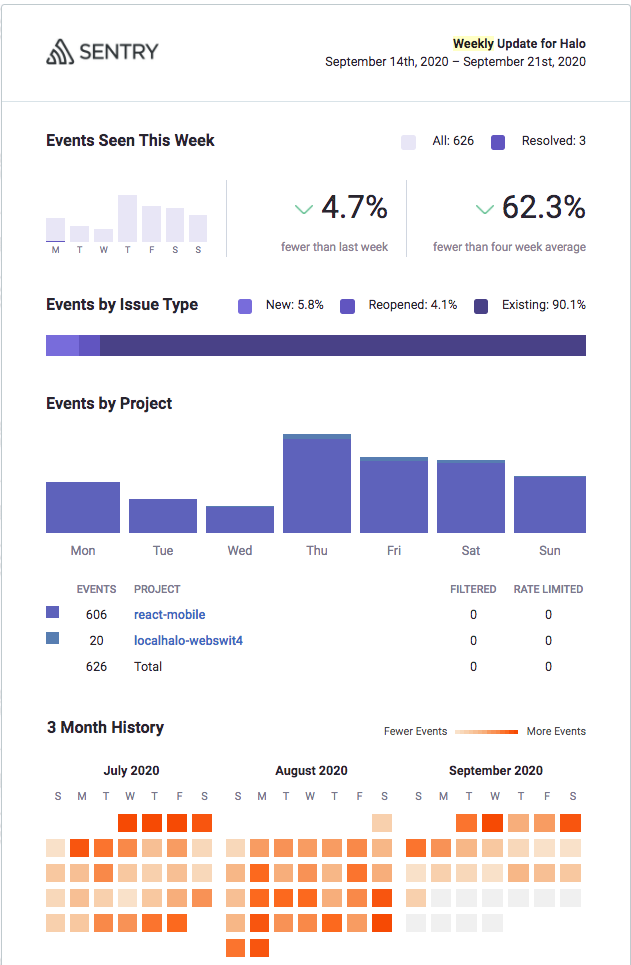
\includegraphics[width=0.42\textwidth]{images/localhalo/sentry-weekly-report-21-Sep-2020.png}
  \end{center}
  \caption{LocalHalo: Sentry weekly report 14 - 21 September 2020}
  \label{fig:localhalo-sentry-weekly-report-21-sep-2020}
\end{wrapfigure}

The weekly reports indicate the majority of detected issues were existing issues, for instance 90.1\% in the week 14 - 21 September 2020, as illustrated in Figure~\ref{fig:localhalo-sentry-weekly-report-21-sep-2020}. This is illustrative, the lowest percentage was 75.6\% and the highest 100\% in the 16 months they have been provided by email. Note the weekly report's analytics combine the react-mobile and website error data, therefore they are not very useful in terms of analytics for solely the mobile app. However, they do include various counts that are specific to the mobile app and therefore useful for a sanity check of the volume of errors on a weekly basis.

\begin{wrapfigure}{R}{0.5\textwidth}
  \begin{center}
    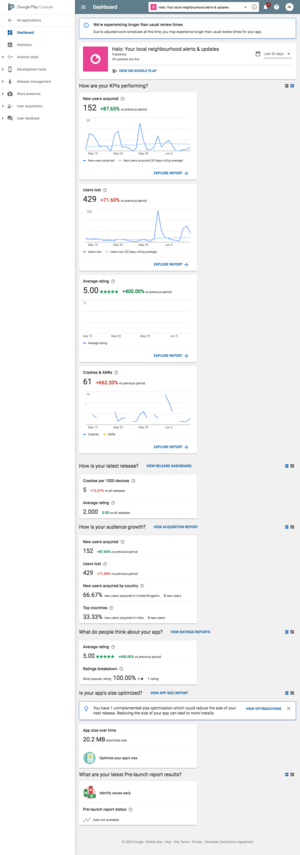
\includegraphics[width=0.42\textwidth]{images/google-play-console/resized-25pct-appdashboardplace_555059634831.png}
  \end{center}
  \caption{Google Play Console Dashboard for LocalHalo Android app}
  \label{fig:gpc-dashboard-for-localhalo-android-resized}
\end{wrapfigure}


\subsection{LocalHalo: Research findings and results from the Case Study}
Android Vitals does report a combined count of crashes and ANRs in the dashboard even for small volumes; however it does not provide any details of these crashes or ANRs in Android Vitals, when the overall volumes are low (low tens of failures per month).

Various flaws in Google Play Console and Android Vitals were corroborated by this case study. The details are aggregated and discussed in \secref{section-google-play-console-case-study}.

Several characteristics of using mobile analytics to improve quality for React Native apps~\footnote{The internals of React Native apps are discussed in an open, online book \url{https://www.reactnative.guide/3-react-native-internals/3.1-react-native-internals.html}.} 
were identified in this case study. For instance, that the native app includes a runtime layer for the React Native code which constrains many of the runtime failures in the app to that runtime rather than exposing them to the platform (Android). Therefore Android does not report on them in Google Play Console or Android Vitals. Developers need to incorporate in-app mobile analytics, such as Sentry, if they wish to discover these runtime errors.

Only the CTO had access to Sentry~\footnote{Evidence: Sentry UI showing team members.} (who else had access to the other analytics tools is not known).

In hindsight, it appears the team did not spot the rapid increase in crash and ANR rates in March 2020 until I contacted them by email when I noticed the high failure rates in Android Vitals when my access to Google Play Console was re-enabled on \nth{26} March 2020. If that's accurate then the team had the opportunity to identify the issue sooner (as indicated in the missing data shown in Figure\ref{fig:sentry-missing-data-march-2020}) up to a week earlier and find ways to mitigate it. 

Data missing from reports from~\nth{17} March to~\nth{25} March 2020 which affected the statistics around the time of the crashes related to Expo. Figure~\ref{fig:sentry-missing-data-march-2020} illustrates the gap across the two weekly reports. 


\subsection{LocalHalo: Outcomes for the company}
The nature of the case study (being remote from the development team, with access limited to two of the mobile analytics services, and correspondence being occasional) meant the outcomes for the company are hard to ascertain. It is clear the founders saw the value in choosing two particular mobile analytics services to help them manage the business and the service their provided to their users. 

Their main focus was to try to grow the business. Ultimately that was not successful, a topic discussed briefly in the next section. The analytics tools continue to report on the app and the website and continue to provide some insights into the reliability of the app and usage of the app.

\subsection{LocalHalo: Discussion}
Even small development teams can and do use multiple mobile analytics services. It was not practical to establish how actively they monitored or responded to the various reports and alerts. The CTO did mention they were working flat out with a small development team at the time; and it is possible they only investigated the app failures related to Expo once they were contacted by the researcher.   

The errors reported by the mobile analytics demonstrate external libraries can adversely affect the reliability of apps. And the combination of a void in the data in Sentry which aligned with the high failure rates being reported in Android Vitals illustrates 1) it is possible for in-app analytics to fail, and even to potentially cause the app to fail; 2) that platform analytics can complement in-app analytics.

There are numerous open questions, for instance: What can developers learn from the various reports provided by Sentry? How does cross-platform development in react-native affect the app reliability? are there crashes that only occur on Android or iOS? What's the correlation between crashes reported in Android Vitals and Sentry?

Note: The founders of local halo indicated~\footnote{Via their respective LinkedIn profiles: \url{https://www.linkedin.com/in/jamesroutledge/} and \url{https://www.linkedin.com/in/andriymarin/}} they are no longer actively involved in this project, and there are confirming indications in sentry.io as the app has not been updated in over a year, in contrast to the many updates they made previously. So even though the app remains online and available, and the analytics continue to report, there is no one actively maintaining the app or dealing with the errors being reported in the analytics.

\newthought{The analytics data provides data for retrospective insights}

Having ongoing long term access to Sentry and their provision of alerts and weekly summary emails provided an unexpected opportunity to use these to obtain some retrospective insights. Some examples include: the discovery that the servers used by the LocalHalo app have been returning 404 response codes for many weeks, and some of the internal development practices including how at least one developer tested the app.


\subsection{LocalHalo: Contributions to the research and where they are located in the rest of this thesis}
This case study contributes to the material on Sentry in \secref{analytics-tools-sentry} and to the material on Google Play Console with Android Vitals in \secref{section-google-play-console-case-study}. It also contributes to the Findings section \secref{findings-section}.


\begin{comment}
I wish we could find out how actively the development team were reading, reviewing and addressing crashes being reported. However, as the project no longer appears to be active that's unlikely to happen.
\end{comment}

\begin{comment}
Extra information available includes:
\begin{itemize}
    \item Their local communities for \href{https://docs.google.com/spreadsheets/d/1iqOvNjRlHIpoRzd61BcBLVkSxGvbta6vrzH2Jgc50aY/htmlview#}{COVID-19 volunteer support communities}.
    \item A social network for neighbors \url{https://ain.ua/en/2019/10/18/localhalo-raises-500k/}
    \item Stack Overflow questions (unpopular and seldom answered) \url{https://stackoverflow.com/questions/tagged/react-native+expo+crash}, a more general search does better \url{https://stackoverflow.com/search?q=\%5Breact-native\%5D+\%5Bexpo\%5D+crash}
    \item Some interesting projects to add device information to React Native apps \url{https://github.com/robinpowered/react-native-vitals} and \url{https://github.com/robinpowered/react-native-device-battery}
    \item A long article, with screenshots in Polish or a similar language on publishing React Native expo apps to both app stores \url{https://pagepro.co/blog/publishing-expo-react-native-app-to-ios-and-android/}
    \item \href{https://gist.github.com/himgupta229/83b4fd61f294020258976e3edb10b16a}{GitHub GIST: JSON for ANR in Sentry}.
    \item Expo recommends Sentry and documents the integration \url{https://docs.expo.dev/guides/using-sentry/}.
    \item Excellent in-depth discussion on what dev's dislike about React Native \href{https://github.com/react-native-community/discussions-and-proposals/issues/64}{GitHub React Native Issue 64}, for instance on debugging exceptions and on lack of resilience to crashes. Facebook provide a similarly detailed reply in \href{https://github.com/react-native-community/discussions-and-proposals/issues/104}{Issue 104 on GitHub}. They followed up this approach in June 2019 in \href{https://github.com/react-native-community/discussions-and-proposals/issues/134}{Issue 134}.
\end{itemize}
\end{comment}